\section*{Примеры работы}

На рисунке~\ref{fig:ex_infix} представлен
пример выполнения программы при вводе
выражения в инфиксной нотации.

\begin{figure}[H]
    \centering
    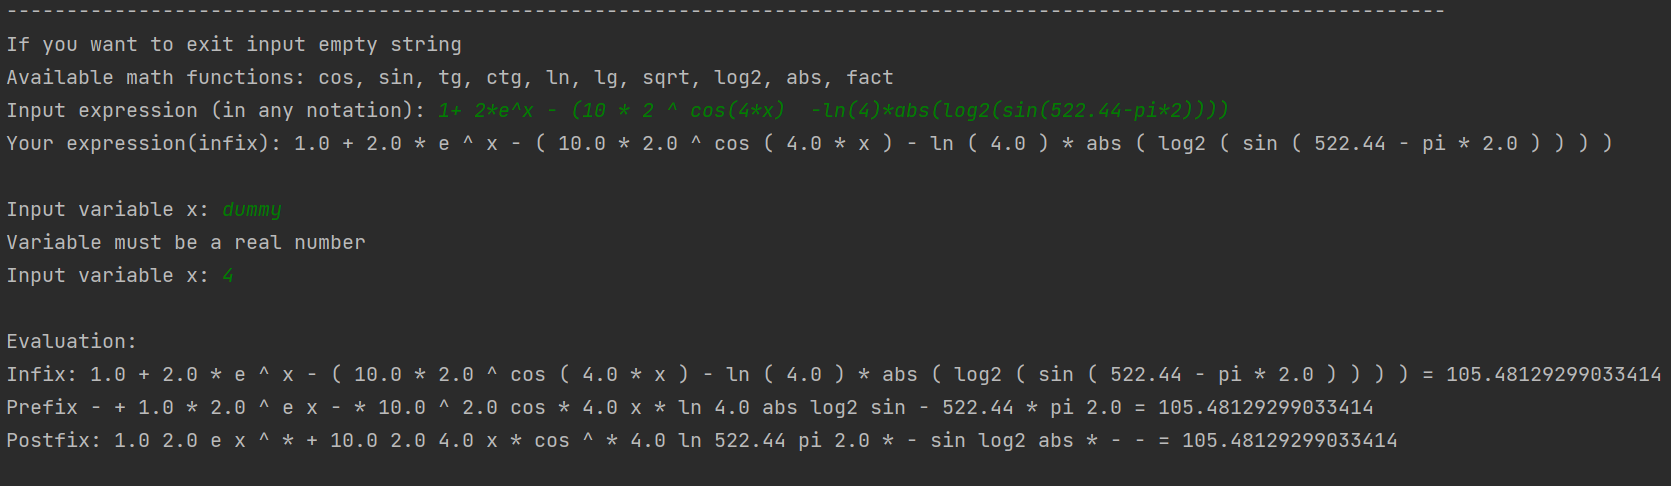
\includegraphics[width=\linewidth]{photo/ex_infix}
    \caption{Пример выполнения для инфиксной нотации}
    \label{fig:ex_infix}
\end{figure}

На рисунке~\ref{fig:ex_prefix} представлен
пример выполнения программы при вводе
выражения в префиксной нотации.

\begin{figure}[H]
    \centering
    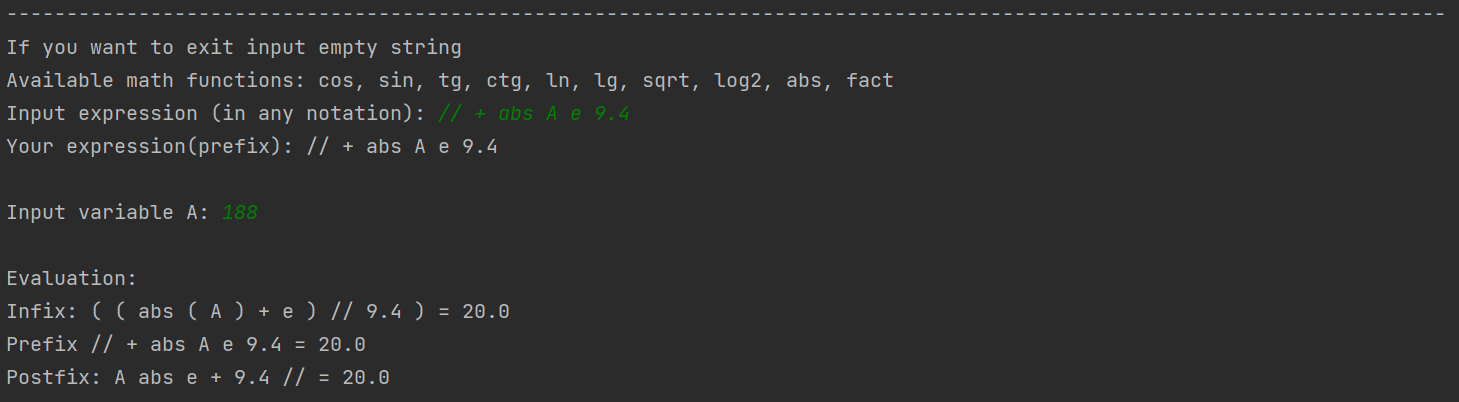
\includegraphics[width=\linewidth]{photo/ex_prefix}
    \caption{Пример выполнения для префиксной нотации}
    \label{fig:ex_prefix}
\end{figure}

На рисунке~\ref{fig:ex_postfix} представлен
пример выполнения программы при вводе
выражения в постфиксной нотации.

\begin{figure}[H]
    \centering
    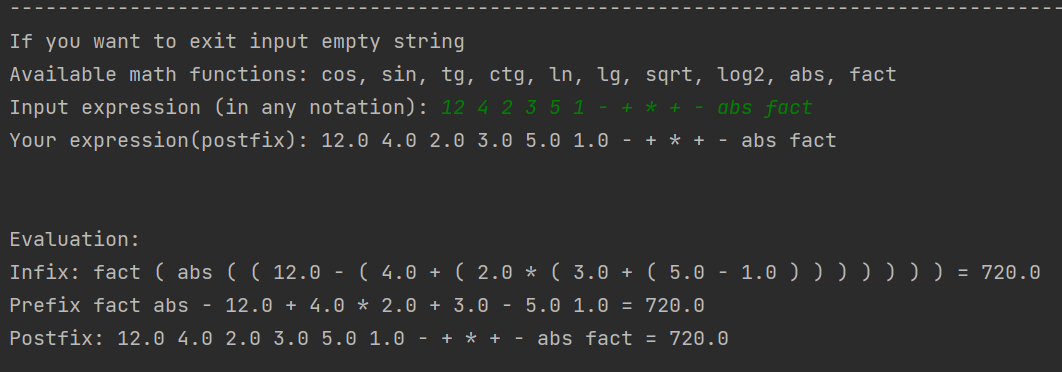
\includegraphics[width=\linewidth]{photo/ex_postfix}
    \caption{Пример выполнения для постфиксной нотации}
    \label{fig:ex_postfix}
\end{figure}

На рисунке~\ref{fig:ex_errors} представлен
пример выполнения программы при некорректном вводе
выражения.

\begin{figure}[H]
    \centering
    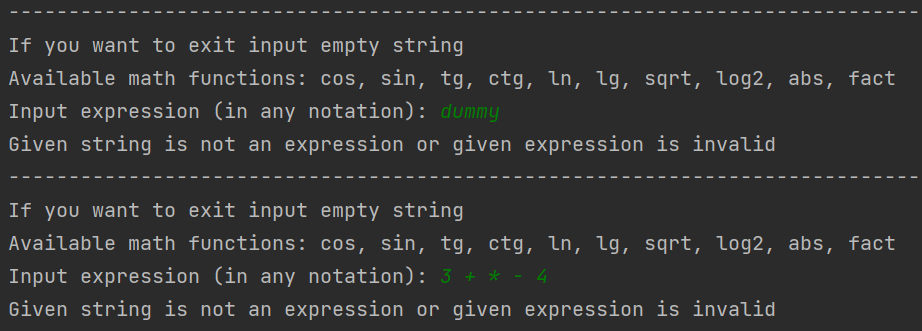
\includegraphics[width=\linewidth]{photo/ex_errors}
    \caption{Пример выполнения при неверных входных данных}
    \label{fig:ex_errors}
\end{figure}